
\documentclass[12pt,a4paper, oneside]{extreport}

%%%%%%%%%% Математика %%%%%%%%%%
\usepackage{amsmath,amsfonts,amssymb,amsthm,mathtools}
% Показывать номера только у тех формул, на которые есть \eqref{} в тексте.
%\mathtoolsset{showonlyrefs=true}
%\usepackage{leqno} % Нумерация формул слева
%\usepackage{tipa} %Для формулки из логитов


\usepackage{hyphenat}

%%%%%%%%%% Шрифты %%%%%%%%
\usepackage[english, russian]{babel} % выбор языка для документа
\usepackage[utf8]{inputenc} % задание utf8 кодировки исходного tex файла
\usepackage[X2,T2A]{fontenc}        % кодировка

\usepackage{fontspec}         % пакет для подгрузки шрифтов
\setmainfont{Times New Roman}       % задаёт основной шрифт документа

\usepackage{unicode-math}      % пакет для установки математического шрифта
%\setmathfont{Asana-Math.otf}    % шрифт для математики

% Конкретный символ из конкретного шрифта
% \setmathfont[range=\int]{Neo Euler}


%%%%%%%%%% Работа с картинками %%%%%%%%%
\usepackage{graphicx}                  % Для вставки рисунков
\usepackage{graphics}
\graphicspath{{images/}{pictures/}}    % можно указать папки с картинками
\usepackage{wrapfig}                   % Обтекание рисунков и таблиц текстом


%%%%%%%%%% Работа с таблицами %%%%%%%%%%
\usepackage{tabularx}            % новые типы колонок
\usepackage{tabulary}            % и ещё новые типы колонок
\usepackage{array,delarray}      % Дополнительная работа с таблицами
\usepackage{longtable}           % Длинные таблицы
\usepackage{multirow}            % Слияние строк в таблице
\usepackage{float}               % возможность позиционировать объекты в нужном месте

\usepackage{booktabs}            % таблицы как в книгах

% Заповеди из документации к booktabs:
% 1. Будь проще! Глазам должно быть комфортно
% 2. Не используйте вертикальные линни
% 3. Не используйте двойные линии. Как правило, достаточно трёх горизонтальных линий
% 4. Единицы измерения - в шапку таблицы
% 5. Не сокращайте .1 вместо 0.1
% 6. Повторяющееся значение повторяйте, а не говорите "то же"
% 7. Есть сомнения? Выравнивай по левому краю!

%  вычисляемые колонки по tabularx
\newcolumntype{C}{>{\centering\arraybackslash}X}
\newcolumntype{L}{>{\raggedright\arraybackslash}X}
\newcolumntype{Y}{>{\arraybackslash}X}
\newcolumntype{Z}{>{\centering\arraybackslash}X}


%%%%%%%%%% Графика и рисование %%%%%%%%%%
\usepackage{tikz, pgfplots}      % язык для рисования графики из latex'a

%%%%%%%%%% Гиперссылки %%%%%%%%%%
\usepackage{xcolor}              % разные цвета

\usepackage{hyperref}
\hypersetup{
	unicode=true,           % позволяет использовать юникодные символы
	colorlinks=true,       	% true - цветные ссылки, false - ссылки в рамках
	urlcolor =blue,         % цвет ссылки на url
	linkcolor=black,        % внутренние ссылки
	citecolor=black,        % на библиографию
	breaklinks              % если ссылка не умещается в одну строку, разбивать ли ее на две части?
}


%%%%%%%%%% Другие приятные пакеты %%%%%%%%%
\usepackage{multicol}       % несколько колонок
\usepackage{verbatim}       % для многострочных комментариев
\usepackage{cmap} % для кодировки шрифтов в pdf

\usepackage{enumitem} % дополнительные плюшки для списков
%  например \begin{enumerate}[resume] позволяет продолжить нумерацию в новом списке

\usepackage{todonotes} % для вставки в документ заметок о том, что  осталось сделать
% \todo{Здесь надо коэффициенты исправить}
% \missingfigure{Здесь будет Последний день Помпеи}
% \listoftodos --- печатает все поставленные \todo'шки



%%%%%%%%%%%%%% ГОСТОВСКИЕ ПРИБАМБАСЫ %%%%%%%%%%%%%%%

%%% размер листа бумаги
\usepackage[paper=a4paper,top=15mm, bottom=15mm,left=35mm,right=10mm,includehead]{geometry}


\usepackage{setspace}
\setstretch{1.33}     % Межстрочный интервал
\setlength{\parindent}{1.5em} % Красная строка.


%\flushbottom       % Эта команда заставляет LaTeX чуть растягивать строки, чтобы получить идеально прямоугольную страницу
\righthyphenmin=2  % Разрешение переноса двух и более символов
\widowpenalty=10000  % Наказание за вдовствующую строку (одна строка абзаца на этой странице, остальное --- на следующей)
\clubpenalty=10000  % Наказание за сиротствующую строку (омерзительно висящая одинокая строка в начале страницы)
\tolerance=1000     % Ещё какое-то наказание.


% Нумерация страниц сверху по центру
\usepackage{fancyhdr}
\pagestyle{fancy}
\fancyhead{ } % clear all fields
\fancyfoot{ } % clear all fields
\fancyhead[C]{\thepage}
% Чтобы не прорисовывалась черта!
\renewcommand{\headrulewidth}{0pt}


% Нумерация страниц с надписью "Глава"
\usepackage{etoolbox}
\patchcmd{\chapter}{\thispagestyle{plain}}{\thispagestyle{fancy}}{}{}


%%% Заголовки
\usepackage[indentfirst]{titlesec}{\raggedleft}
% Заголовки по левому краю
% опция identfirst устанавливает отступ в первом абзаце



% В Linux этот пакет сделан косячно. Исправляет это следующий непонятный кусок кода.
\makeatletter
\patchcmd{\ttlh@hang}{\parindent\z@}{\parindent\z@\leavevmode}{}{}
\patchcmd{\ttlh@hang}{\noindent}{}{}{}
\makeatother


% Редактирования Глав и названий
\titleformat{\chapter}
{\normalfont\large\bfseries}
{\thechapter }{0.5 em}{}

% Редактирование ненумеруемых глав chapter* (Введение и тп)
\titleformat{name=\chapter,numberless}
{\centering\normalfont\bfseries\large}{}{0.25em}{\normalfont}

% Убирает чеканутые отступы вверху страницы
\titlespacing{\chapter}{0pt}{-\baselineskip}{\baselineskip}

% Более низкие уровни
\titleformat{\section}{\bfseries}{\thesection}{0.5 em}{}
\titleformat{\subsection}{\bfseries}{\thesubsection}{0.5 em}{}

\titlespacing*{\section}{0 pt}{\baselineskip}{\baselineskip}
\titlespacing*{\subsection}{0 pt}{\baselineskip}{\baselineskip}


% Содержание. Команды ниже изменяют отступы и рисуют точечки!
\usepackage{titletoc}

\titlecontents{chapter}
[1em] %
{\normalsize}
{\contentslabel{1 em}}
{\hspace{-1 em}}
{\normalsize\titlerule*[10pt]{.}\contentspage}

\titlecontents{section}
[3 em] %
{\normalsize}
{\contentslabel{1.75 em}}
{\hspace{-1.75 em}}
{\normalsize\titlerule*[10pt]{.}\contentspage}

\titlecontents{subsection}
[6 em] %
{\normalsize}
{\contentslabel{3 em}}
{\hspace{-3 em}}
{\normalsize\titlerule*[10pt]{.}\contentspage}


% Правильные подписи под таблицей и рисунком
% Документация к пакету на русском языке!
\usepackage[tableposition=top, singlelinecheck=false]{caption}
\usepackage{subcaption}


\DeclareCaptionStyle{base}%
[justification=centering,indention=0pt]{}
\DeclareCaptionLabelFormat{gostfigure}{Рисунок #2}
\DeclareCaptionLabelFormat{gosttable}{Таблица #2}

\DeclareCaptionLabelSeparator{gost}{~---~}
\captionsetup{labelsep=gost}

\DeclareCaptionStyle{fig01}%
[margin=5mm,justification=centering]%
{margin={3em,3em}}
\captionsetup*[figure]{style=fig01,labelsep=gost,labelformat=gostfigure,format=hang}

\DeclareCaptionStyle{tab01}%
[margin=5mm,justification=centering]%
{margin={3em,3em}}
\captionsetup*[table]{style=tab01,labelsep=gost,labelformat=gosttable,format=hang}


% межстрочный отступ в таблице
\renewcommand{\arraystretch}{1.2}



% многостраничные таблицы под РОССИЙСКИЙ СТАНДАРТ
% ВНИМАНИЕ! Обязательно за CAPTION !
\usepackage{fr-longtable}



%Более гибкие спсики
\usepackage{enumitem}
% сообщаем окружению о том, что существует такая штук как нумерация русскими буквами.
\makeatletter
\AddEnumerateCounter{\asbuk}{\russian@alph}{щ}
\makeatother


%%% ГОСТОВСКИЕ СПИСКИ

% Первый тип списков. Большая буква.
\newlist{Enumerate}{enumerate}{1}

\setlist[Enumerate,1]{labelsep=0.5em,leftmargin=1.25em,labelwidth=1.25em,
	parsep=0em,itemsep=0em,topsep=0ex, before={\parskip=-1em},label=\arabic{Enumeratei}.}


% Второй тип списков. Маленькая буква.
\setlist[enumerate]{label=\arabic{enumi}),parsep=0em,itemsep=0em,topsep=0.75ex, before={\parskip=-1em}}


% Третий тип списков. Два уровня.
\newlist{twoenumerate}{enumerate}{2}
\setlist[twoenumerate,1]{itemsep=0mm,parsep=0em,topsep=0.75ex,, before={\parskip=-1em},label=\asbuk{twoenumeratei})}
\setlist[twoenumerate,2]{leftmargin=1.3em,itemsep=0mm,parsep=0em,topsep=0ex, before={\parskip=-1em},label=\arabic{twoenumerateii})}


% Четвёртый тип списков. Список с тире.
\setlist[itemize]{label=--,parsep=0em,itemsep=0em,topsep=0ex, before={\parskip=-1em},after={\parskip=-1em}}


%%% WARNING WARNING WARNIN!
%%% Если в списке предложения, то должна по госту стоять точка после цифры => команда Enumerate! Если идет перечень маленьких фактов, не обособляемых предложений то после цифры идет скобка ")" => команда enumerate! Если перечень при этом ещё и двууровневый, то twoenumerate.




%%%%%%%%%% Список литературы %%%%%%%%%%

%\usepackage[%
%backend=biber, %подключение пакета biber (тоже нужен)
%bibstyle=gost-numeric, %подключение одного из четырех главных стилей biblatex-gost
%sorting=ntvy, %тип сортировки в библиографии
%]{biblatex}

\usepackage[backend=biber,style=gost-numeric, maxbibnames=9,maxcitenames=2,uniquelist=false, babel=other]{biblatex}



% Справка по 4 главным стилям для ленивых:
% gost-inline  ссылки внутри теста в круглых скобках
% gost-footnote подстрочные ссылки
% gost-numeric затекстовые ссылки
% gost-authoryear тоже затекстовые ссылки, но немного другие

% Подробнее смотри страницу 4 документации. Она на русском.

% Ещё немного настроек
\DeclareFieldFormat{postnote}{#1} %убирает с. и p.
\renewcommand*{\mkgostheading}[1]{#1} % только лишь убираем курсив с авторов


\addbibresource{diploma11.bib} % сюда нужно вписать свой bib-файлик.



% Этот кусок кода выносит русские источники на первое место. Костыль описали авторы пакета в руководстве к нему. Подробнее смотри:
% https://github.com/odomanov/biblatex-gost/wiki/Как-сделать%2C-чтобы-русскоязычные-источники-предшествовали-остальным
\DeclareSourcemap{
	\maps[datatype=bibtex]{
		\map{
			\step[fieldsource=langid, match=russian, final]
			\step[fieldset=presort, fieldvalue={a}]
		}
		\map{
			\step[fieldsource=langid, notmatch=russian, final]
			\step[fieldset=presort, fieldvalue={z}]
		}
	}
}

\DefineBibliographyStrings{english}{%
	pages = {P\adddot},
	number = {№},
}



\begin{document} % Начала документа

\thispagestyle{empty} % Чтобы избежать нумерации титульника

% Если для какой-то страницы хочется сделать своё уникальное оформление, как например для титульника или списка литературы, то можно использовать окружение \begingroup ... \endgroup.
\begingroup
\setstretch{1}   % Убираем полторашные интервалы на титульнике
\begin{center}
\small \bfseries Федеральное государственное бюджетное образовательное учреждение высшего образования

<<РОССИЙСКАЯ АКАДЕМИЯ НАРОДНОГО ХОЗЯЙСТВА и\\ ГОСУДАРСТВЕННОЙ СЛУЖБЫ \\
при Президенте Российской Федерации>>

\vspace{2ex}

\bfseries
Институт ЭМИТ
ЭКОНОМИЧЕСКИЙ ФАКУЛЬТЕТ

Напривление  ЭКОНОМИКА И ФИНАНСЫ
\end{center}

\vfill


\noindent  Группа ЭО-15-01
\hfill
\parbox[t]{20em}{\centering
Кафедра микроэкономики

\mbox{ }

\textbf{Допустить к защите}

заведующий кафедрой микроэкономики

\mbox{ }

\rule{8em}{0.5pt} М.И. Левин

\mbox{ }

<<\rule{2em}{0.5pt}>> \rule{5em}{0.5pt} 2018 г. }

\mbox{ }

\mbox{ }

%\begin{center}\bfseries
%ВЫПУСКНАЯ КВАЛИФИКАЦИОННАЯ РАБОТА

\mbox{ }

\begin{center}
{\large
Разработка и исследование моделей роста \\ при условии ограниченности ресурсов }
\end{center}

\vfill

\noindent\normalsize
студент-бакалавр

\noindent
Касьянова Ксения Алексеевна 
\hfill /\rule{6em}{0.5pt}/\rule{6em}{0.5pt}/

\hfill\makebox[13em]{\hfill\footnotesize (подпись) \hfill\hfill (дата) \hfill}

\noindent
научный руководитель 

\noindent
д.э.н. Левин Марк Иосифович 
\hfill /\rule{6em}{0.5pt}/\rule{6em}{0.5pt}/

\hfill\makebox[13em]{\hfill\footnotesize (подпись) \hfill\hfill (дата) \hfill}

%\noindent
%консультант
%
%\noindent
%д.э.н., профессор Петров Петр Петрович
%\hfill /\rule{6em}{0.5pt}/\rule{6em}{0.5pt}/
%
%\hfill\makebox[13em]{\hfill\footnotesize (подпись) \hfill\hfill (дата) \hfill}

\vfill

\begin{center}
\normalsize \bfseries МОСКВА \\ 2018 г.
\end{center}
\endgroup



%%%%%%%%%%%%%%%%%%% ОГЛАВЛЕНИЕ %%%%%%%%%%%%%%%%%%%%%%%%%%%%%%%%%%%%%%

\tableofcontents  % Команда, которая создаёт оглавление



%%%%%%%%%%%%%%%%%%%% ВВЕДЕНИЕ %%%%%%%%%%%%%%%%%%%%%%%%%%%%%%%%%%%%
\chapter*{Введение}
\addcontentsline{toc}{chapter}{Введение}

Природные ресурсы играют важную роль в экономическом росте
и благосостоянии страны. Они являются одним из основных факторов производства, технологического прогресса, международной  торговли,
а также влияют на уровень жизни в стране, ее  социальную и политическую сферы.



Экономический рост в основном определяется технологическим прогрессом,
который предполагает  производство большего  количества товаров и услуг при использовании того же числа единиц   труда, капитала, энергии и сырья. 




Сложная взаимосвязь между дефицитом природных ресурсов и экономическим ростом  страны  приводит к противоречивым выводам относительно того,  как, положительно  или отрицательно,    сказывается   дефицит природных ресурсов на экономическом росте.



Также не понятно, какой  способ позволяет наилучшим  образом  измерить дефицит ресурса. Какие из этих показателей -  цена на ресурс, удельные издержки добычи,  ресурсная рента, стоимость  энергии и эластичность  замещения - точнее  всего описывают нехватку  природных ресурсов.




В данной работе исследуются  теории экономического  роста при ограниченности натуральных ресурсов. 


Цель работы: изучить, как проблема нехватки ресурсов 
% или роста цен на ресурсы  
вписывается в существующие теории экономического  роста,  для  получения более рациональной  оценки  экономического риска.
%Целью данной работы является изучение  теоретических основ ..., методики разработки и оценки ..., анализ эффективности ... .



%Актуальность рассматриваемой темы заключается в том, что ... занимает центральное место в процессе обоснования и выбора возможных вариантов ... в операции с ... . Эффективность ... характеризуется ..., отражающих соотношение затрат и результатов в зависимости от ... .



Достижение поставленной цели предполагает постановку и решение следующих задач:

%Вопросы, представляющие интерес при исследовании  экономической модели: 
\begin{itemize}
	\item Определить теоретические основы моделирования  экономического роста
	\item Рассмотреть существующие модели, учитывающие использование агентами запасов невозобновляемого  ресурса
	\item Выбрать спецификацию модели на основе проведенного анализа
	\item Изучить, как введение в модель неопределенности изменит оптимальные пути и стабильность системы 
	%\item Возможно ли имитировать заданную эмпирическую закономерность с использованием исследуемой  модели? 
	\item Проанализировать, как изменятся свойства стохастического процесс для вектора  эндогенных переменных при модификации вектора экзогенных переменных
	\item С помощью методов численного программирования, определить   как на динамику модели влияют импульсы от шоков	
	%Какая часть в этой закономерности объясняется  импульсами от  шоков? 
	%Как изменяется стохастический процесс для вектора  эндогенных переменных при модификации вектора экзогенных переменных? 
	%\item Можно ли уменьшить несоответствие между теоретической моделью и данными путем введения в модель каких-либо  структурных  особенностей? 
	%\item Можно ли использовать неоклассическую  модель  роста для объяснения общего для многих стран эмпирического  факта, что относительная дисперсия  потребления к выпуску меньше единицы, тогда как относительная дисперсия  инвестиций к выпуску значительно выше единицы? 
	%\item Насколько точно  можно  воспроизвести  численные значения этих дисперсий с учетом только технологических шоков?
	%\item Насколько вырастет качество подгонки модели при добавлении неопределенности  в предпочтения отдельных потребителей? 
%	\item  %Стандартная модель роста предсказывает высокую корреляцию между часами работы и производительностью, что противоречит эмпирическим наблюдениям.
	%Улучшит  ли качество модели  добавление в нее  дополнительного сектора отвечающего за  накопление человеческого капитала? 
\end{itemize}


Теоретической  основой исследования послужили работы ученых в области динамического моделирования, стохастического оптимального контроля, теоретического и эмпирического  анализа моделей роста.  














Данная работа состоит из введения, двух глав основной части, заключения и приложений.
В первой  главе рассматриваются основные направления в моделировании экономического роста.
Во второй главе проводится анализ модели роста ресурсозависимой экономики сначала аналитическими математическими методами и численного программирования.

В данной работе мной был проведен анализ моделей роста (Приложение А), на основе которого была выбрана модель, наилучшим образом описывающая потребление ограниченного ресурса. В дополнение результатов, уже полученных авторами модели, мною были подтверждены и прокомментированы некоторые условия (пункт 2.3), которые у авторов работы шли без доказательства.   Самый главный вывод, сделанный мной, был получен в ходе  анализа данной модели  в отношении  динамики  запаса ресурса. На эти детали авторы работы свое внимание не обратили, но я считаю, что он как раз показывает  всю важность применения методов стохастического анализа при моделировании запасов ограниченного ресурса. Эти выводы представлены в пункте 2.5., а также визуализированы мной с помощью MATLAB (пункт 3.2)  


%В заключении даются выводы по проделанному анализу, полученные в ходе исследования.%Данная работа состоит из введения, основной части, заключения и приложений.
%Во введении  формулируются цель и задачи исследования, обосновывается актуальность выбранной темы. 
%Основная часть состоит из ... глав.
%Первая глава раскрывает понятие бизнес-проекта, цели его разработки, методики оценки проектов, факторы, влияющие на эффективность инвестиций.
%Во второй главе проводится анализ деятельности предприятия, а также описывается сущность бизнес-плана предприятия.
%В третьей главе проводится оценка экономической эффективности проекта, с помощью различных методов оценки, оценивается чувствительность бизнес-проекта к внешним и внутренним факторам.




\chapter{Модели роста}


Одной из функций экономической теории является создание искуственных моделей,   на основе которых можно было бы при минимальных затратах оценить влияние дорогостоящих экспериментов по внедрению каких-либо политик.  Подвергая экономическую модель  шокам, можно быть на достаточном уровне  уверенным  в том, что в реальности экономики  отреагируют так же. Проведем анализ того, как изменялся подход к изучению экономического роста в соответствие с требованиями времени.



\section{Обзор литературы}


На протяжении века ученые рассматривали вопрос экономического роста страны.  Делая акценты на различные аспекты они определяли различные факторы роста. 

%история
Так например, для изучения долгосрочного экономического роста используется неоклассическая модель роста, также известная как модель экзогенного роста. Эта теория впервые была разработана Солоу (1956) и Суоном (1956).  В ней норма сбережения задается экзогенно.  
Кстати, в последующей  статье Солоу (1957) объясняет рост производительности  американской экономики,  оценивая показатели технологического прогресса  как остатки по  капиталу и труду  для временных рядов  за  1909-1949 гг.
Далее Рамсеем (1928) развивается  модель, в которой  норма сбережения может быть получена эндогенно при решении проблемы максимизация полезности домашних хозяйств. Касс (1965) и Купманс (1965) модифицируют модель Рамсея путем включения в нее темпов роста населения и технического прогресса. Брок и Мирман (1972) добавляют  неопределенность в модель Рамсея.
Кидланд и Прескотт (1982) применяют стохастическую модель  оптимального  роста  к данным по США, чтобы  изучить какая часть колебаний в бизнес-циклах объясняется технологическими  шоками.  Их модель лежит в основе     теории реального делового цикла.

%RBC?
%В некоторых версиях моделей бизнес-циклов утверждается, что совокупное потребление, доходы и инвестиции коинтегрированные переменные.
Некоторые традиционные модели бизнес-циклов предполагают, что шоки спроса, которые являются основной  причиной  экономических колебаний,  временные, поэтому темпы  экономического роста в долгосрочном периоде   возвращаются к естественному уровню. 



%end 
В 1980-е годы повысился  интерес как к роли человеческого капитала, так  и к причинам  технологического прогресса. Были разработаны эндогенные модели долгосрочного роста, в рамках которых  технический прогресс связывался  с различными  экономическими факторами. 


%человеческий капитал
Т. Шульц первым выдвинул идею инвестиций в «человеческий капитал» в попытке объяснить  различия в доходе на душу населения
по странам. 



В модели Ромера (1986)  создание фирмой новых технологий  приводит к  положительным экстерналиям, увеличивая  производственные возможности других фирм.
В модели Лукаса (1988), основанной на работе  Узавы (1965), внимание уделяется  человеческому капиталу, а не физическому, в  предположении что накопление человеческого капитала и технологий являются  одним и тем же.
Разница между двумя группами теорий заключается в том, что эндогенный рост в теории Ромера  вызван накоплением технологий (или знаний), которое является неконкурентным и частично исключаемым благом. В теории Лукаса эндогенный рост идет за счет неуменьшающейся предельной отдаче  от накопления  человеческого капитала. 





Обзор основных теорий экономического роста представлен в таблице в приложении.





\section{Различия теории  экзогенного и эндогенного экономического роста}


%N 
Важнейшей особенностью  неоклассической теории  является предположение об уменьшающейся  отдаче от  капитала и труда. 

Существует три основных положения теории неоклассического роста.
\begin{itemize}
	\item в долгосрочном  устойчивом состоянии, рост выпуска определяется темпами роста эффективности  рабочей силы  и не зависит от нормы сбережения 
	\item уровень дохода на душу населения зависит от нормы сбережения, положительно связан с отношением сбережений к инвестициям  и отрицательно связаны со скоростью роста населения
	\item 	 существует обратная связь между отношением капитала к труду и производительностью капитала (в предположении об  идентичных предпочтения и технологиях в разных странах)
\end{itemize}


Теория неоклассического роста предсказывает абсолютную  конвергенцию для стран  с равными нормами  сбережений, темпами  роста населения и с доступом к одной и той же технологии, а также условную конвергенцию для стран с разными нормами  сбережений или темпами  роста населения устойчивое состояние  отличается, но темпы роста в конечном итоге сходятся.



%n vs e history
Основная критика неоклассической теории роста,  заключается в том, что 
она говорит о том, что темпы экономического роста и норма сбережения некоррелированы в устойчивом состоянии.


В теории эндогенного роста делается попытка объяснить 
устойчивые темпы роста  производственных показателей на душу населения, а также различия в темпах роста для разных стран.




Существует несколько  типов факторов в  моделях эндогенного роста: 
\begin{itemize}
	\item внешние эффекты, связанные  с  накоплением  капитала  и  знаний
	\item  накопление  человеческого капитала 	
	\item   продолжающийся рост числа  производительных «проектов», способствующих созданию дополнительных проектов
\end{itemize}


Теория эндогенного роста предсказывает, что высокая сберегательная ставка приводит к высоким темпам роста без конвергенции.


%solow vs lucas
Так например, в модели  Солоу, политика по увеличению человеческого капитала  будет оказывать временное воздействие на экономический рост при  переходе  к новому  устойчивому состоянию,  в то время   как в модели Лукаса  говорится о   эффекте постоянного роста. 



%критика
Одним из основных недостатков эндогенных теорий роста является то, что ей не удается объяснить условную конвергенцию, подтвержденную  в эмпирической литературе.


Одним из интересных вопросов явлется изучение влияние динамики населения на экономический рост. 
Примером изменения динамики населения может быть миграция.
Миграция по сути является инвестициями в будущее, позволяющим покинуть   бедный  рынок труда, заплатив сегодня    фиксированную стоимость переезда в надежде на более высокую заработную плату завтра.

%MIGRATION IN NEOCLASSICAL GROWTH MODELS
В стандартной неоклассической односекторной модели роста, миграция происходит вследствие разницы в  реальных заработных платах между регионами  и способствует в итоге  выравниванию цены на факторы производства. 
Соответственно миграция в краткосрочном периоде  способствует  конвергенции  различий реальных заработных плат по регионам и странам, в то время как в долгосрочном периоде  миграция может повлиять на реальный рост заработной платы за счет изменений в технологиях. 
%Эмпирически подтверждено, что чистая миграция не влияет на прирост доходов на душу населения в краткосрочном периоде, но оказывает влияние   на рост в долгосрочном периоде. 

\begin{figure}[h!]
	\centering
	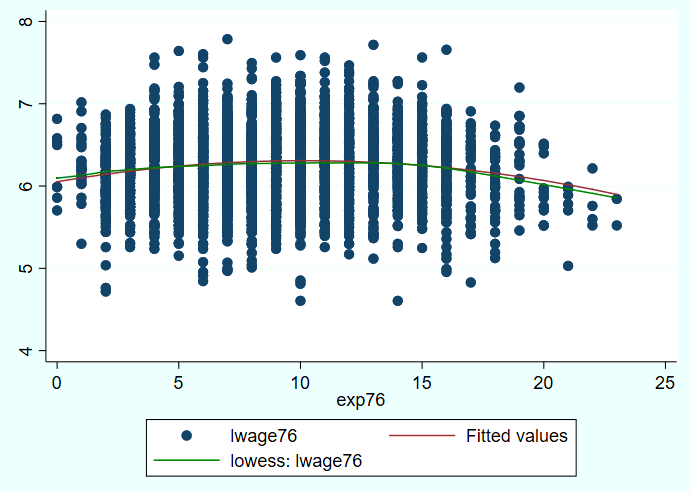
\includegraphics[width=0.7\linewidth]{screenshot004}
	\caption[Эффект миграции в неоклассическоц модели роста]{Эффект миграции: миграция  способствует  конвергенции  различий реальных заработных плат по регионам и странам, $n_1, n_2 $ - темпы роста населения в регионах до миграции,  $m $ - темп миграции. }   
	\label{fig:screenshot004}
\end{figure}



На графике видно, что миграция при неоклассических предпосылках приводит к  совершенной конвергенции.
Хотя здравый смысл подсказывает, что миграция только увеличивает разницу в темпах роста экономик различных стран. Для изучения этого вопроса больше подходит эндогенная модель роста, 
поскольку  миграционные потоки скорее будут влиять не только на скорость изменения темпов роста населения, а еще и на скорость  технологического прогресса  и внутреннее равновесие, в результате чего разрыв между странами становится еще больше.




%\section{Модели с человеческим капиталом}

%The models of endogenous growth typically consider innovation and learning as drivers of growth. It is also widely accepted that human capital is an important input for innovation. Human capital can be accumulated through learning-by-doing or schooling that uses existing human capital and the additional human capital then also becomes an input into production. There is also path dependence: the cost of innovation falls permanently when the stock of knowledge becomes larger. In this case a more developed region or country has an advantage over others and therefore attracts new firms and workers. As a result of the path dependency, agglomeration might occur. 

%Human capital is defined as consisting of the abilities, skills and knowledge of particular workers, and is thus rival and excludable. Furthermore, although human capital is embodied in workers and hence represents in fact a specific kind of labour, it is treated as a second type of capital in analogy to physical capital. This definition of human capital has two major effects within the modelling framework: firstly, introducing human capital implies that the sum of shares of output paid to capital of both kinds is raised. Secondly, devoting more resources to the accumulation of either type of capital increases the amount of output that can be produced in the future.

%Some  forms  of investment in people: Schooling; Training programs; Experience (on the job training); Health; Migration 

%On a theoretical level, the three models presented above differ significantly from each other. Their main distinguishing features are summarized in table. Given these differences, it is interesting that the empirically testable predictions which can be derived from the models do not vary as radically as the theoretical debate might lead one to expect.
%	
%	\begin{table}[H]
%		\caption{Differences between models of economic growth which include human capital}\label{tab}
%		\small\centering\setlength{\extrarowheight}{0.25em}
%		\begin{tabular}%{\linewidth}
%			{   >{\footnotesize}p{10em} 
%				>{\centering\footnotesize}p{10em} 
%				>{\centering\footnotesize}p{10em} 
%				>{\centering\footnotesize\arraybackslash}p{10em} }\hline
%			
%			&  Augmented Solow model & 		 Lucas model & 	 Romer model \\\hline
%			
%			Human capital is accumulated by… & investing a fraction of income & spending a fraction of time acquiring skills & not modeled \\ 
%			Technology for production of human capital &
%			same production function for C, K and H &
%			separate sector for production of H using only human capital &
%			not modeled \\
%			Role of human capital &
%			input in production &
%			input in production of Y and H &
%			input in production of Y and A \\
%			Growth rate determined…
%			&outside of the model
%			&within the model
%			&within the model
%			\\Determinant of long-run growth
%			&Exogenous technological change
%			&rate of human capital accumulation
%			&stock of human capital
%			\\Effect of a permanent change in the variable governing the accumulation of human capital
%			&level effect (relevant variable: $ s_H $ )
%			&rate effect (relevant variable: $ 1-u^* $)
%			&rate effect (though not explicitly modeled)
%			\\Effect of a one-off increase in the stock of human capital
%			&level effect
%			&level effect
%			&rate effect \\\hline
%			
%			
%		\end{tabular}
%	\end{table}






\section{Факторы ограничивающие экономический рост }


%limits on growth
В неоклассической теории   концепции  физического  предела роста  уделяется недостаточное внимание, в предположении, что рынок и технологические достижения  позволят задействовать новые ресурсы и создать замещение производственных факторов. При этом   полностью исключаются  ограничения, вызванные  политическими, психологическими и социальными причинами. В классической теории, наоборот,  учитывается   множество ограничений для роста, включая демографические, экологические и социальные факторы.


В теории Адама  Смита  неявно обсуждается демографический предел роста, поскольку труд является автономным производственным фактором предполагается свободно доступным, а капитал и технология эндогенно созданы через вложение прибыли.
Модель работает в предположении, что рост численности населения  будет достаточным для того,  чтобы  ограничение рабочей силы на выходе не было значимым.


В модели Рикардо исследуются  ограничения   на производительность земли и рост населения.
Он использует  принципа уменьшении предельной ренты от  земли,  приравненное  к производительности земли, а также    закона Рикардо о заработной плате, утверждающем, что  население будет расти до тех пор, пока ставка  заработной платы не достигнет  уровня прожиточного минимума. Таким образом, через  прожиточный минимум выражается  демографические ограничения на предложения рабочей силы.  
При выполнении  этих принципов  каждая дополнительная единица  выпуска потребует больше единиц  капитала и труда для производства. Поскольку темпы роста рабочей силы снижаются,  производство достигает "плато", где прибыль равна  нулю, в то время как предельный продукт труда приближается к установленному законодательством прожиточному минимуму.


Томас Мальтус создал  модель  динамического роста, в которой  истощение  ресурсов идет за счет роста населения. 
В этой модели  наблюдается  конвергенция   уровня  доходов  на душу населения. 
В долгосрочной перспективе улучшения  уровня жизни наблюдаться не будет, пока  не будет введены  ограничения на рост населения.
Рост населения является не  причиной, а  конечным результатом  экономического роста, который происходит вследствие   пропорционального увеличения богатства.  


Далее при построении модели мы будем рассматривать  ресурс как  фактор, способный повлиять на темпы  экономического роста.




\chapter{Разработка и исследование модели ресурсозависимой экономики}


%?
Многие страны с низким уровнем дохода  зависят  от своей ресурсной базы:  они  имеют достаточно  большие запасы земли и ресурсов  плохого качества,  низкую  производительность  сельского хозяйства, деградации земель и ограниченный потенциал развития населения.   
Первоначальные  ограниченные   запасы ресурсов  при высоких уровнях  ставки дисконтирования, связанной  с временными предпочтениями, может привести к неустойчивым траекториям роста ресурсозависимой экономики. 



Существуют разные мнения о  влиянии дефицита природных  ресурсов на экономический  рост. Например, любой недостаток энергетических ресурсов может привести к  шоку предложения и спровоцировать рост цен на нефть, в  результате чего  экономический рост замедляется. 



%немножко воды
Одним их ресурсов, который может ограничивать экономический  рост является вода. В большинстве стран сегодня эта проблема не возникает,   но чрезвычайная нехватка воды может спровоцировать  снижение темпов   роста, хотя инвестиции  в увеличение запасов водных ресурсов уравновешивает это влияние. 
Нехватка  воды, нужной  для производства пищи  или  в  национальных масштабах также влияет и на  развитие спроса. 
Нехватка воды для развития сельского хозяйства также требует изменений существующих  институтов.


Для моделирования риска нехватки  воды,   используя, например,  модель общего равновесия,  также  требуется  анализ международной торговли  продуктами,  для производства которых требуется вода. 
Влияние на международную торговлю тем больше, чем жестче   ограничения на водный ресурс или чем больше  воды требуется  в производстве.







\section{Динамика запаса ресурсов}

Одной из важных проблем является правильный выбор  спецификации  стохастического процесса, определяющего  динамику запаса ресурсов.


Запас невозобновляемого ресурса  не может увеличиваться с течением времени. На норму его доходности  влияют   предельная производительность, изменяющиеся физические характеристики ресурса и любые изменения рыночной стоимости. 
При прочих равных условиях технологический прогресс должен сократить затраты на добычу природных ресурсов. Рыночная стоимость дефицитного ресурса должна увеличиваться
со временем, поскольку  ресурс становится все более дефицитным, пока если альтернативы ему  найден.


%Population laws
Скорость изменения ресурса в принципе не является  детерминистической величиной, поскольку она подверженна  многим  факторам  и неопределенностям,  системным и связанным с  воздействиями  окружающей среды. 






Для моделирования  неопределенности, мы можем разложить ее на детерминистическую и стохастическую компоненту 

\begin{equation}\label{key}
\dfrac{dx(t)}{x(t)} = R(x(t), t )  dt + V (x(t),t ) dB(t)
\end{equation}

где $ x (t) $ - запас ресурса,   $ R $ - средняя скорость изменения  $ x (t) $ в момент времени $ t $, $ V $ - стандартное отклонение скорости изменения  $ x (t) $ в момент времени $ t $, $ dB (t) $ -   является стандартным броуновским движением с нормальным распределением  $ N (0, dt) $.


\begin{table}[H]
	\caption{Способы   моделирования   ресурса}\label{tab}
	\small\centering\setlength{\extrarowheight}{0.25em}
	\begin{tabular}%{\linewidth}
		{   >{\footnotesize}p{13em} 
			>{\centering\footnotesize}p{5em} 
			>{\centering\footnotesize}p{5em} 
			>{\centering\footnotesize\arraybackslash}p{16em} }\hline
		
		& 	$ R (x (t), t) $ &  $  V (x (t), t) $  & SDE \\		\hline
		
		Экспоненциальная модель роста	& 	$ \mu $  &  $  \sigma $ & 	 $ dx(t) = \mu x(t)dt + \sigma x(t)dB(t) $\\
		
		Логистическая модель 	&  $ b + ax(t)  $ & $  \sigma x(t) $ & $  dx(t) = x(t) ( [b + ax(t)]dt + \sigma x(t) dB(t) ) $ 
		\\  
		
		
		Процесс с квадратным корнем	&  $  \mu  $ &  $ \dfrac{ \sigma}{\sqrt{x(t)}} $ & $ dx(t) = \mu x(t)dt + \sigma \sqrt{x(t)} dB(t) $\\
		Процесс возвращающий среднее 	&$  \dfrac{(\mu − x(t))}{x(t)} $ & $ \dfrac{ \sigma}{\sqrt{x(t)}} $
		&
		$dx(t)=(\mu − x(t))dt +   \sigma \sqrt{x(t)} dB(t)  $ 
		\\
		$ \theta $ - процесс		&  $  \mu $ & $  \sigma(x(t))^{\theta−1} $ &  
		$ dx(t) = \mu x(t)dt + \sigma(x(t))^{\theta} dB(t) $ \\
		\hline	
	\end{tabular}
\end{table}


Предположим, что  скорость роста постоянна $ \mu $. Запишем выражение  в виде обыкновенного дифференциального уравнения  (ОДУ): 

\begin{equation}\label{key}
\dfrac{dx(t)}{dt} =  \mu  x(t)
\end{equation}

Решением этого  линейного ОДУ  является функция   экспоненциального роста  (или уменьшения) запаса  ресурса:  
\begin{equation}\label{key}
x(t) = x(0)e^{\mu t}  
\end{equation}
, где $ x(0) $ - начальный запас  ресурса   в момент времени $ t = 0 $.


Как результат мы имеем: 

\begin{itemize}
	\item Если $ \mu > 0 $, то  $ x (t) \rightarrow \infty $ запас ресурса  будет расти экспоненциально быстро. 
	\item Если $ \mu < 0 $, то  $  x (t) \rightarrow 0 $ запас ресурса  будет уменьшаться  экспоненциально быстро.
	\item Если $ \mu = 0 $, то  $  x (t) = x (0) $ для любого  $ t $, т.е.  запас ресурса стационарен. 
\end{itemize}

Если мы учитываем   неопределенность, то имеем: 

\begin{equation}\label{eq1}
\dfrac{dx(t)}{x(t)} =  \mu  dt +\sigma dB(t)
\end{equation}

По формуле Ито:

\begin{equation}\label{eq2}
d \ln(x(t) )  =  0 + \dfrac{1}{x(t) } d x(t) -  \dfrac{1}{2} \dfrac{1}{x^2(t)} (d x(t)) ^2 =  \dfrac{d x(t)}{x(t) }   -  \dfrac{\sigma^2}{2}  d t 
\end{equation} 


Откуда, интегрируя \eqref{eq2} с учетом \eqref{eq1}, имеем: 

\begin{equation}\label{eq3}
\int_{0}^{t} \dfrac{dx(t)}{x(t)} = \ln\left( \dfrac{x(t)}{x(0)}  \right) + \dfrac{\sigma^2  t}{2}    =   \mu  t +\sigma B(t) 
\end{equation}


И, проэкспоненциировав \eqref{eq3}, получаем  явное решение:

\begin{equation}\label{it}
x(t) =  x(0) \exp \left(    \left(  \mu - \dfrac{\sigma^2}{2} \right)    t +\sigma B(t) \right) 
\end{equation}



Свойства этого решения отличаются от детерминистического случая: 

\begin{itemize}
	\item Если $ \mu > 0.5 \sigma^2  $, то  $ x (t) \rightarrow \infty $ запас ресурса  будет расти экспоненциально быстро с вероятностью 1. 
	\item Если $ \mu <  0.5 \sigma^2 $, то  $  x (t) \rightarrow 0 $ запас ресурса  будет уменьшаться  экспоненциально быстро с вероятностью 1.
	\item Если $ \mu =  0.5 \sigma^2 $, то учитывая, что по закону повторного логарифма   $ \limsup_{t \rightarrow \infty} \dfrac{B(t)}{\sqrt{2t \ln \ln t } } = 1  $ и  $ \liminf_{t \rightarrow \infty} \dfrac{B(t)}{\sqrt{2t \ln \ln t } } = -1  $ ,  то  $ \limsup_{t \rightarrow \infty}  x (t) = \infty $, а  $ \liminf_{t \rightarrow \infty}  x (t) = 0 $   с вероятностью 1. 
\end{itemize}

В частности, главным отличием является   случай, когда $ 0 < \mu <  0.5 \sigma^2  $. В детерминистической модели запас ресурса бы  бесконечно увеличивался, в то время как в стохастической он бы снижался экспоненциально    быстро. Откуда мы получаем важный вывод: добавление неопределенности в модель может привести к выводу о том, что ресурс будет полностью  исчерпан.    


Также одним из важных выводов является то, что при использовании логистической модели мы предполагаем, что запас ресурса будет изменяться согласно следующему закону

\begin{equation}\label{key}
x(t) = \dfrac{b}{-a + e^{-bt}\dfrac{b + a x(0)}{x(0)}} 
\end{equation} 
откуда с помощью нехитрых подсчетов мы выводим время $ T $, при которым запас ресурса становится бесконечно   большим (при $a>0, b>0  $).   

При этом добавление стохастического параметра приводит к тому, что при  любых коэффициентах запас ресурса не устремится к бесконечности.

\section{Выбор спецификации модели}


%стохастика
В работах  семидесятых годов  многие экономисты (Brock and Mirman (1972), Lucas (1976), Sargent (1979)  среди многих других) показали необходимость формулировать макроэкономические вопросы в динамической, стохастической установке.

%On uncertainty
Стохастические свойства экономических переменных определяют их поведение. Изучение их  важно для построения эконометрических моделей, интерпретации результатов и прогнозирования. 
Любое эконометрическое исследование временных рядов требует анализа стохастических свойств переменных. 
Стоит отметить, что свойства экономических переменных, присущих  временным рядам,   играют  важную роль применительно к исследованию макроэкономических моделей. Как мы  увидели в предыдущем пункте поведение любых переменных сильно различается в детерминистической и стохастической установке.  


Стохастические шоки могут  повлиять  на правила политики, предпочтения агентов,  технологии, и т.д. Если  экономические агенты принимают решения в условиях неопределенности, то  их выбор сегодня  влиет на их  возможные наборы в будущем, что надо учесть с помощью  стохастического   динамического моделирования при анализе  последствий  экономической политики. 
Вне зависимости от вида  инноваций технологический прогресс обычно описывается  Пуассоновским потоком.
Именно поэтому нам интересно рассмотреть стохастическую динамическую модель экономического роста. 





%стохастическая модель
Теоретическую динамическую стохастическую модель можно рассматривать как набор ограничений на  распределение вероятностей  вектора соответствующих переменных.  
Эти ограничения могут вытекать  из аналитической структуры модели (функциональной спецификации технологий, предпочтений, устаревания производительного и человеческого капитала, и т. д.),  значений параметров,
и  многомерного распределения вероятностей векторного случайного процесса, заданного для моделирования экзогенных шоков.

Аналитическим решением такой модели является распределение вероятности векторного стохастического процесса. В случае модели общего экономического равновесия ищется динамическое стохастическое общее равновесие (DSGE) модели. Некоторые характеристики распределения вероятностей могут быть получены из аналитического решения. Однако  очень часто решение не может быть получено аналитически, поэтому приходится использовать  методы математического моделирования,  которые дают приближения, в виде распределения частот для векторного стохастического процесса. 



Пусть  скорость изменения  природного ресурса описывается  стохастическим   дифференциальным   уравнением:
\begin{equation}\label{key}
d R (t) = r_0 R (t) (dt + dz (t)) 
\end{equation}
где $ r_0 $ - первоначальная скорость    пополнения ресурса, заданная экзогенно, $ dz(t)  $  -   независим во времени, нормально распределен $ N(0, \sigma_{z}^{2}) $ 

Выпуск  зависит от эффективности использования ресурса, которая в свою очередь зависит от возможностей технологического прогресса от которого также зависит скорость пополнения ресурса. 
Производственная функция,  таким образом, должна  удовлетворять следующему стохастическому дифференциальному уравнению:
\begin{equation}\label{key}
dY (t) = \alpha K(t) ( dt  + dy (t)) 
\end{equation}
где $ K(t) $ - используемый  природный ресурс, $ a > r_0 $ -
скорость   пополнения   эксплуатируемых природных ресурсов, заданный  также экзогенно,  $ dy(t) $   -   независим во времени, нормально распределен $ N(0, \sigma_{y}^{2}) $ 

Общий запас ресурса $ X(t) $ в таком случае: 
\begin{equation}\label{eqq1}
 X (t) = R (t) - K(t)
 \end{equation}
 Пусть ресурс распределяется на $ \eta_K + \eta_R = \dfrac{K(t)}{X(t)} + \dfrac{R(t)}{X(t)}  = 1 $ 
В таком случае требуется из множества возможных распределений ресурса выбрать оптимальное,   позволяющее сохранить ресурс и  максимизировать  общую ожидаемую полезность.
\begin{equation}\label{tt}
\max_C E_0 \int_{0}^{+ \infty}  e^{-\beta t} \dfrac{C(t)^{1-\rho}}{1-\rho}  dt 
\end{equation}
где $ E_t $ - математическое ожидание в  момент времени $ t \geq 0 $  по  вероятностной мере, $ \beta > 0  $  - дисконтирующий  фактор, $ \rho > 0  $   -  параметр отношения к риску.


Из \eqref{eqq1} $  X (t) $ изменяется согласно  следующему уравнению:
\begin{equation}\label{cc2}
dX(t) = (\alpha K (t) + r_0 R(t) - C(t)) dt + \alpha K(t) dy + r_0 R(t) dz
\end{equation}
где $ X (0) = x $. 

$ X (t) $ - переменная состояния, потребление $ C (t) $ и  запас природного ресурса $  R (t) $ - переменные контроля.



Задача оптимизации в таком случае выглядит следующим образом: 

\begin{flalign}
& V(X(t), t)  =  \max_{C, \eta_K, \eta_R} E_t \int_{t}^{+ \infty}  e^{-\beta (s - t)} \dfrac{C(s)^{1-\rho}}{1-\rho}  ds    \\ 
s.t.: \   &  dX (t) = \left( \alpha \eta_K +  r_0 \eta_R  - \dfrac{C(t)}{X(t)}\right)   X(t) dt + X(t) dw  \nonumber \\
 & \eta_K + \eta_R =  1 \nonumber
\end{flalign}
где $ V(t, X) $ - целевая функция, $  dw = \alpha \eta_K dy +  r_0 \eta_R dz $, причем $ \sigma_{w}^{2} = \alpha^{2} \eta_K^{2} \sigma_{y}^{2} +  r_0^{2} \eta_R^{2} \sigma_{z}^{2}  $ 

По лемме Ито: 
\begin{equation}\label{key}
L_X (V (X, t)) = V_t  +  \left( \alpha \eta_K +  r_0 \eta_R  - \dfrac{C(t)}{X(t)}\right)   X(t) V_X + \dfrac{1}{2} \sigma_{w}^{2}  X^{2}(t) V_{XX} 
\end{equation}

Тогда соответствующий Гамильтониан: 
\begin{equation}\label{key}
\mathcal{H} = e^{-\beta t} \dfrac{C(t)^{1-\rho}}{1-\rho}     + L_X + e^{- \beta t} \lambda (1 - \eta_K -  \eta_R ) 
\end{equation}

Соответствующие условия первого порядка: 
\begin{flalign}
& \dfrac{\partial \mathcal{H}}{\partial C(t)} =   e^{-\beta t} C(t)^{-\rho} - V_X = 0 \label{eqq2} \\
&  \dfrac{\partial \mathcal{H}}{\partial \eta_K} =  \alpha X V_x + X^{2}(t) \alpha^{2} \eta_K \sigma_{y}^{2} V_{XX}  - e^{-\beta t } \lambda  = 0 \label{eqq3}  \\
&  \dfrac{\partial \mathcal{H}}{\partial \eta_R} = r_0  X V_x + X^{2}(t) r_0^{2} \eta_R \sigma_{z}^{2} V_{XX}  - e^{-\beta t } \eta  = \lambda   \label{eqq6}  \\ 
&    \dfrac{\partial \mathcal{H}}{\partial \lambda} = 1 - \eta_K -  \eta_R = 0 \label{eqq4}
\end{flalign}

Условие из уравнения  Беллмана: 
\begin{equation}\label{eqq5}
\mathcal{H} = e^{-\beta t} \dfrac{C(t)^{1-\rho}}{1-\rho}     + L_X  = 0
\end{equation}

Условие \eqref{eqq2} говорит о том, что предельная полезность потребления дисконтированная  по времени определяет скорость пополнения с учетом  уравнения  Беллмана \eqref{eqq5}. Из уравнений  \eqref{eqq3}, \eqref{eqq6}, \eqref{eqq4} определяем  оптимальное распределение ресурса.

Потребление будет считаться по следующей формуле:
\begin{equation}\label{cc}
C(t) = (\delta (1-\rho) )^{-\dfrac{1}{\rho} } X(t) 
\end{equation}
где $ \delta $ - параметр,  эндогенно  определяемый из равновесия в системе 

Решив систему уравнений получаем:
\begin{equation}\label{eqeq}
\eta_K = \dfrac{\alpha - r_0 + \rho r_0^2 \sigma_{z}^2}{\rho( \alpha^{2}  \sigma_{y}^{2} +  r_0^{2} \sigma_{z}^{2}   )}
\end{equation} 

Откуда получаем, что если $ \dfrac{a - r_0}{\rho} <  \alpha^{2}  \sigma_{y}^{2}   $,   то доля  используемого  ресурса менее единицы. Рациональный  социальный планировщик  должен приостановить добычу ресурса, позволив ему накопиться естественным образом, чтобы  удовлетворить потребности человечества в будущем.

Из уравнения \ref{eqeq} получаем
\begin{equation}\label{eqeq1}
\dfrac{\partial \eta_K}{\partial \sigma_{y} } = - \alpha^2 \dfrac{\alpha - r_0 + \rho r_0^2 \sigma_{z}^2}{\rho( \alpha^{2}  \sigma_{y}^{2} +  r_0^{2} \sigma_{z}^{2}   )^2} <0 
\end{equation}
\begin{equation}\label{eqeq2}
\dfrac{\partial \eta_K}{\partial \sigma_{z} } = - \alpha^2 \dfrac{\alpha - r_0 + \rho r_0^2 \sigma_{z}^2}{\rho( \alpha^{2}  \sigma_{y}^{2} +  r_0^{2} \sigma_{z}^{2}   )^2} > 0 
\end{equation}
Эти неравенства показывают, рост неопределенности по выпуску  ведет к росту доли  используемого ресурса, а  увеличение неопределенности по  запасу ресурсов  ведет к снижению  доли используемого   ресурса.

Из уравнения Беллмана \eqref{eqq5} получаем: 
\begin{equation}\label{cc1}
\dfrac{C}{X} = \dfrac{2\beta + \rho(1-\rho)\sigma_{w}^2 + 2 (\rho - 1 ) (\alpha \eta_K + r_0 \eta_R)}{2\rho} 
\end{equation}
Из этого уравнения мы видим, что влияние  $ \sigma_{y}^2 $ и $  \sigma_{z}^2 $ на  долю потребляемого ресурса в запасе  ресурса $ X(t) $ неоднозначно. 


Из уравнений \eqref{cc} и  \eqref{cc1}, мы можем вывести значение параметра $ \delta $:
\begin{equation}\label{tt2}
\delta = \left( \dfrac{C}{X}\right)^{-\rho}  (1-\rho)^{-1} = \dfrac{1}{1-\rho} \left(\dfrac{2\beta + \rho(1-\rho)\sigma_{w}^2 + 2 (\rho - 1 ) (\alpha \eta_K + r_0 \eta_R)}{2\rho}  \right)  ^{-\rho}
\end{equation}


Из уравнения \eqref{cc2}  получим  ожидаемую скорость роста $ \phi $:
\begin{equation}\label{сс3}
\phi = \alpha\eta_K + r_0 \eta_R - \dfrac{C(t)}{X(t)}
\end{equation}
Откуда мы видим, что ожидаемые темпы роста ресурса  эндогенно определяются как усредненное  распределение  ресурса $ \alpha\eta_K + r_0 \eta_R $ за вычетом доли потребленного ресурса $  \dfrac{C(t)}{X(t)}  $. 
	
	Объединив \eqref{cc3}  с \eqref{eqq5} получим формулу ожидаемого темпа роста ресурса: 
	\begin{equation}\label{key}
	\phi = \dfrac{\alpha \eta_K + r_0 \eta_R - \beta}{\rho} + \dfrac{1}{2} (\rho -1	) \sigma_{w}^2
		\end{equation}

Аналогично потреблению, влияние $ \sigma_{y}^2 $ и $  \sigma_{z}^2 $   на темпы роста ресурса   неоднозначно, поскольку он  зависит и от других  факторов, шоков, скоростей прироста ресурса, межвременных предпочтений, отношения к риску.

В стационарное состоянии  системы параметры, описывающие распределение  ресурса  \eqref{eqeq1}, c учетом ограничения \eqref{eqq4} на параметры,  доля потребления ресурса   \eqref{cc1}  и  ожидаемый  темп прироста  ресурса являются константами. 
Это утверждение говорит о том, что неизвлеченные  ресурсы, используемые ресурсы, потребляемые  ресурсы  и сам ресурс будут расти с постоянным  ожидаемым темпом роста.  

Тогда 
\begin{equation}\label{key}
dX = \phi Xdt q + Xdw
\end{equation}

В этом случае по лемме Ито  запас природного ресурса определяется как:  
\begin{equation}\label{qqq}
x(t) =  x(0) \exp \left(    \left(  \phi - \dfrac{\sigma^2_w}{2} \right)    t +  w  \right) 
\end{equation}
где $ w = w(t) - w(0) = \sigma^2_w B(t) $, $ B(t) $ - стандартное броуновское движение. 

 


\section{Вывод условия трансверсальности}


Условие трансверсальности (из \eqref{tt} и \eqref{tt2} )
\begin{equation}\label{key}
\lim_{t \rightarrow \infty}  e^{-\beta t} v(X(t), X(t+1))  X(t)  =  
\lim_{t \rightarrow \infty}  e^{-\beta t}  \dfrac{C(t)^{1-\rho}}{1-\rho} X = 
\lim_{t \rightarrow \infty}  e^{-\beta t} \delta X^{1-\rho} = 0 \end{equation}
будет выполняться  тогда и только тогда, когда  $ 1-\rho \left( \phi - \dfrac{\sigma_{w}^2}{2}\right)  - \beta  < 0 $.

По  сути условие трансверсальности говорит нам о том, что текущее приведенное потребление ресурса в бесконечно далеком периоде равняется нулю. Другими словами, потребление в следующем периоде  $ X(t+1 )  $ не должно расти быстрее, чем   предельное приращение   $ e^{-\beta t} v(X(t), X(t+1))   $. Это условие говорит  о том, что не будет наблюдаться чрезмерного потребления  в будущем, поскольку, если агент сегодня потребляет слишком мало, а в будущем слишком много, то он не ведет себя оптимально. 



\section{Исследование коэффициентов}


Поскольку аналитически определить влияние различных параметров сложно,  примем $ \sigma_{w}^2 = 0 $  и проанализируем частный случай. 

Тогда в стабильном состоянии мы имеем:
\begin{flalign}
& \eta_K = \dfrac{\alpha - r_0 }{\rho  \alpha^{2} \sigma_{y}^{2}}\\ 
& \dfrac{C}{X} = \dfrac{2\beta +  2 (\rho - 1 ) (\alpha \eta_K + r_0 \eta_R)}{2\rho}  \\ 
& \phi = \dfrac{\alpha \eta_K + r_0 \eta_R - \beta}{\rho} 
\end{flalign}


Тогда мы можем говорить о влиянии различных параметров системы на изучаемые переменные.   

Например,  ожидаемый темп роста запаса ресурса $ \phi  $   и доля используемых  ресурсов $ \eta_K $ отрицательно зависят от дисперсии производительности $ \sigma_{y} $,  а доля потребления ресурса $ \dfrac{C}{X} $  отрицательно связаны с ней  при $ \rho > 1 $ и положительно при $  0 < \rho < 1 $. 

Темп роста $ \phi $ также положительно связан со скоростью пополнения используемого ресурса $ r_0 $,    доля используемых ресурсов $ \eta_K $  положительно связаны с ожидаемым темпом пополнения запаса ресурса $ \phi $, если $  r_0 < \alpha < 2r_0 $, отрицательно, если $  \alpha > 2r_0 $. Отношение потребления к ресурсу   $ \dfrac{C}{X} $  отрицательно зависит от   темпов пополнения запаса ресурса $ \phi $, если $  0 < \rho  < 1  $, положительно, если $  \rho  > 1  $.


Для того чтобы изучить влияние этих параметров на систему в остальных случаях, когда  $ \sigma_{w}^2 \neq 0 $,     нам потребуются  численные методы.  
 
 
 
\section{ Вывод} 
 
 Мы знаем, что запас нашего ресурса ведет себя согласно формуле \eqref{qqq}.  
 
 \begin{equation*}\label{qqq}
 x(t) =  x(0) \exp \left(    \left(  \phi - \dfrac{\sigma^2_w}{2} \right)    t +  w  \right) 
 \end{equation*}
 
 
 С помощью методов стохастического анализа мы можем провести анализ, аналогичный анализу модели  из  предыдущего пункта \eqref{it}. 
 
 Заметим важные свойства, на которые не обратили внимание авторы модели, но которые важны для понимания, того, как будет вести себя запас ресурса. 
 
 Если ожидаемая скорость роста запаса ресурса  выше чем $ \frac{1}{2} $ дисперсии запаса  ресурса,  то запас ресурса  будет расти экспоненциально быстро с вероятностью 1.   Если ниже, то запас ресурса  будет уменьшаться  экспоненциально быстро с вероятностью 1.
 
 Еще раз отметим, что введение неопределенности в систему, а именно $ dz $ и $  dy  $,    приводит к тому, что  в    случае, когда $ 0 < \phi <  0.5 \sigma^2_w  $,   в детерминистической модели мы бы спрогнозировали    бесконечный рост ресурса,  в то время как в стохастической, наоборот,  он бы был исчерпан.  
 
 Это еще раз подчеркивает важность введения стохастически заданных величин при    анализе и прогнозировании резервов истончаемых ресурсов.  
 
 
 
 
\chapter{Применение численных  методов}



%on numerical simulation
Для решения проблем динамической	  стохастической оптимизации экономистами используются такие  математические методы решения, как  динамическое программирование с использованием уравнения Беллмана,  принципа максимума Понтрягина или аппроксимации цепей Маркова по методу Кушнера.

Но широкий класс  моделей   может  быть проанализированы только с помощью методов  численного моделирования. 
Использование численных методов значительно расширило класс  вопросов, адресуемых при анализе динамических стохастических экономических моделей.
Использование численных методов позволяет откалибровать значения параметров, смоделировать  и интерпретировать  предполагаемые результаты, что позволяет провести  анализ действенности политики и точнее охарактеризовать исследуемую модель. 



Численное решение представляет собой набор временных рядов  для каждого  из переменных  модели, удовлетворяющий всем условиям модели в    каждом периоде. 
Моделирование же по сути является  процессом нахождения численного  решения  для каждой   реализации вектора  стохастического процесса экзогенных шоков. 
Обычно значения параметров  изменяются для различных  решениям. Находя реализации модели большое чило  раз, мы можем довольно точно аппроксимировать распределение вероятностей вектора  стохастического процесса исследуемых  переменных.


Калибровка модели, с  технической точки зрения,   заключается в привязывании параметрам  численных значений для последующих  генераций реализаций переменных модели. В некотором смысле  калибровка аналогична оценке параметров. Тем не менее, связь  между результатами калибровки  и  методами классической статистики, оценки и тестирования гипотез точно  не определена.

%калибровка
Стандартный метод калибровки модели использовался впервые в работе Kydland и Prescott (1982).  Этот довольно неформальный метод позволял оценить  значения  структурных параметров так, чтобы установившиеся устойчивые состояния   наиболее релевантных переменных соответствовали  наблюдаемым эмпирически выборочным средним.
В частности, такая процедура стала стандартной для   количественного анализа  модели общего  динамического стохастического равновесия (DSGE).










Есть несколько пунктов, на которые  надо обратить внимание  до того, как  мы перейдем к самому анализу модели:

\begin{itemize}
	\item Потребность в использовании численных методов  мотивирована  нелинейностью  функций, описывающих  переменные состояния и оптимального  решения 
	\item  Численное решение   равновесной модели имеет смысл получить, если предполагается, что  конкурентное  равновесие  и распределение  ресурсов при  централизованном планировании  эквивалентны. Численные методы могут использоваться  не только в  моделях, в которых  выполняется вторая теорема  благосостояния.
	\item  Численные  методы  позволяют  бороться  с гетерогенностью агентов, тем самым модель  не ограничивается выбором репрезентативного агента 
	\item   Численные методами  также   могут быть   оценены  модели с эндогенными  ожиданиями.
	
\end{itemize}








Итак, рассматривая экономики  как находящиеся  в их стохастическом устойчивом состоянии, можно сказать, что они  стабильно  колеблются  вокруг детерминистического стационарного состояния, что  может как провоцировать экономический рост, так и нет. 

В моделях экзогенного роста детерминистическое стабильное состояние   может быть достигнуто,  если вероятность появления случайного шока равно  нулю  в любом  периоде  и на скорости роста эндогенных переменных  наложены  определенные ограничения. 
В случае  эндогенного роста,  полученные численным методом  временные ряды не будут стационарными даже после детрендирования. 
Несмотря на это, в большинстве статей проводится  анализ стабильного состояния  моделей эндогенного роста, поэтому выводы в основном относятся к  изменениям в долгосрочном периоде.


Нам интересно оценить последствия  различных политик, которые применяются, как правило, в  экономиках, находящихся  вне стационарного состояния.  Для того, чтобы проанализировать, что происходит с переходной экономикой переходящей  в  устойчивое состояние,  требуются  инструменты для решения нелинейных, динамических стохастических моделей, позволяющие охарактеризовать  переход экономики из одного состояния в другое, тем самым определить  последствия  вмешательства государства,  не ограничивая анализ только долгосрочными последствиями. 



Итак, применим  MATLAB   для решения стохастической динамической модели роста, описанной  в предыдущем пункте,  прогнав полученное уравнение \eqref{qqq} 10000 раз и посчитав среднее.



\begin{figure}[h!]
	\centering
	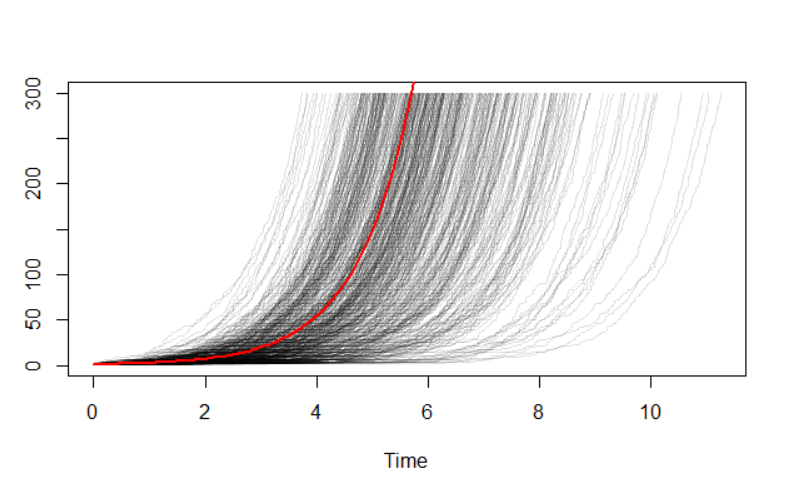
\includegraphics[width=0.7\linewidth]{eosGJ}
	\caption{Экспоненциальный рост запаса ресурса}
	\label{fig:eosgj}
\end{figure}





% intro - bayes
%We are increasingly going to reach such contingent conclusions. Some researchers view such relativity as a weakness of economic analysis, suggesting that it would better to discuss policy in simpler models, even if they miss some interesting feature, since they allow for neater conclusions. The opposite is, however, more likely to be true. Economists may have been too ambitious in attempting to reach statements that would always be true, regardless of the type of economy being studied. In characterizing optimal policy as a function of the structure of the economy (source of shocks, structural parameter values, etc..) we are borrowing from Bayesian statisticians, who sometimes aim at providing their readers with a sort of catalogue, that de…nes the mapping between input (the structure of the economy) and output (the speci…cation of optimal policy). Did we really believe that a similar kind of policy would be optimum for a variety of widely di¤erent economies and for any conceivable policy environment?





\section{Стабильность модели}

Стабильность является важной характеристикой численного решения. Анализ стабильности  стохастической динамической модели отличается от  ее детерминистической  версии. Он также отличается в  эндогенных  и экзогенных моделях роста.

Если решение  нелинейной  стохастической системы, для которой общие аналитические условия неизвестны, стабильно, то  все, что мы можем сделать, это построить и проанализировать  наилучшую линейную аппроксимацию. 

После получения конкретной   реализации  вектора состояний и контроля можно  определить  свойства их совместного распределения: выборочное среднее, стандартные отклонения, дисперсию, простые и частные автокорреляционные функции, коэффициенты корреляции, взаимнокорреляционные функции,  представление в виде векторной авторегрессии (VAR), импульсные характеристики, декомпозиция дисперсий и т. д. 


\section{ Визуализация полученных выводов}



Смоделировав поведение запаса ресурса с помощью MATLAB мы можем убедиться, что ресурс будет вести себя согласно теоретическим выводам.

Предположим, что $ x(0) = 10, \phi = 0.8, \sigma_w = 0  $.  Тогда мы имеем дело с детерминистическим случаем, запас нашего ресурса будет экспоненциально увеличиваться, если 
\[  \phi > 0  \] 



\begin{figure}[h]
	\centering
	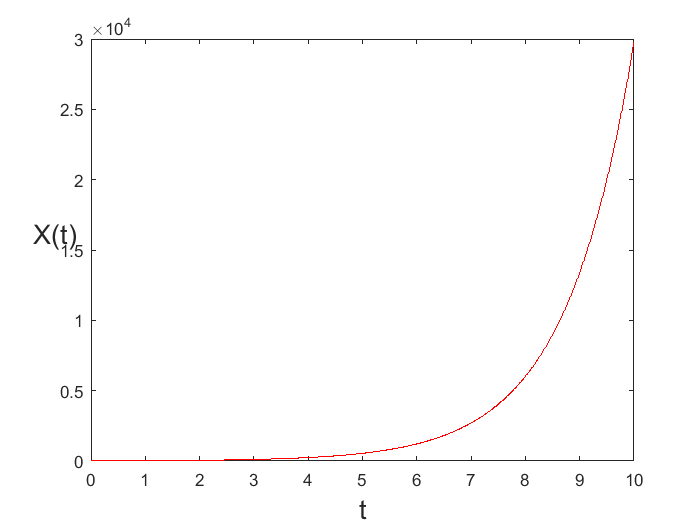
\includegraphics[width=0.5\linewidth]{3}
	\caption{Экспоненциальный рост запаса ресурса в детерминистическом случае при $  \phi = 0.8, \sigma_w = 0  $ }
	\label{fig:eosgj}
\end{figure}

\newpage

Аналогичную картину мы видим при  $  \phi = 0.8, \sigma_w = 0.6  $.  Тогда мы имеем дело со стохастическим  случаем, когда

\[  \phi >  0.5 \sigma^2_w   \]

Запас нашего ресурса будет также экспоненциально увеличиваться. 


\begin{figure}[h]
	\centering
	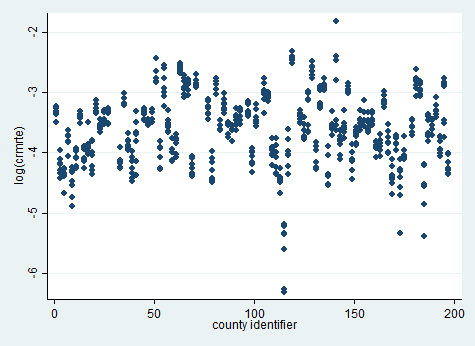
\includegraphics[width=0.8\linewidth]{4}
	\caption{Экспоненциальный рост запаса ресурса в стохастическом  случае при $  \phi = 0.8, \sigma_w = 0.6  $ }
	\label{fig:eosgj}
\end{figure}

\newpage

Если же мы задаем  $  \phi = 0.8, \sigma_w = 4  $, то теперь мы видим случай, когда:

\[  0 < \phi <  0.5 \sigma^2_w  \]



\begin{figure}[h]
	\centering
	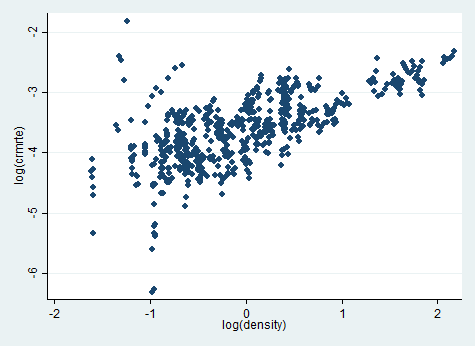
\includegraphics[width=0.8\linewidth]{2}
	\caption{Экспоненциальный рост запаса ресурса в стохастическом  случае при $  \phi = 0.8, \sigma_w = 4  $ }
	\label{fig:eosgj}
\end{figure}


Таким образом мы продемонстрировали, что при одинаковом ожидаемом темпе роста запаса ресурса $ \phi $,  но разных показателях волатильности  ресурса мы  имеем противоположные результаты. Это еще раз убеждает нас в том, что важна точная  оценка коэффициентов в стохастических моделях, поскольку неопределенность может неожиданным образом повлиять на результаты модели.   


%for intro
%How does one define a concept in the random case analogous to the deterministic steady state? In implementing this research program and in the mathematical analysis, Mirman (1972, pp. 224) ¯rst assumed that his random variables A(t) - technology shocks" - were independent, identically distributed in discrete time, and at any time independent of the capital labor ratios, k(t); further, it was assumed that the shocks A(t) were always strictly positive and ¯nite, (bounded away from both zero and in¯nity). To further simplify the analysis and avoid the possibility of a steady state at either zero or in¯nity, the technology (production function) was assumed to satisfy the simple derivative conditions of Inada (satis¯ed by the CD technology). With these assumptions, Mirman used mathematical techniques similar to those in the theory of Markov chains to establish the stochastic generalization of the Solow growth model by showing the existence, uniqueness, and stability of stationary probability measures. With his assumptions, he proved that a stationary measure will always exist, and the stationary measure will be unique if the recurrent states all communicate and admit no cyclically moving subsets. Stability meant that iterates (sequences) of the transition probability tend to a unique asymptotic (time invariant) probability measure (distribution). The tools of the Markov processes were used to demonstrate such stability (convergence) to the unique stationary (steady-state) distribution of the capital labor ratio. 





%on stochastics and use of num comp
%Linear-quadratic optimization problems, those in which the objective function is quadratic and restrictions are linear, will produce a quadratic Lagrangian and hence, first order conditions will be linear in state and decision variables. State variables are predetermined each period, being either past decision variables or variables exogenous to the decision-maker. In a model in which different economic  agents solve their own optimization problem, variables which are decisions for one agent may be state variables for other agents in the economy. In a deterministic setup, first order conditions, together with budget constraints and the assumed mechanism for price formation will form a linear system each period, with as many equations as decision variables, providing the optimal values for the decision variables as a function of the values of the state variables. It is necessary, however, to check that transversality conditions hold when they are necessary for optimality, as it is the case in most economic models.







%Dynare Solow

%Since marginal rate of savings is constant, the response of consumption just mirrors the response on income.  There is a quick response from capital accumulation to increased productivity; once the shock is gone, capital adjusts slowly towards steady state. The initial jump in capital is due to additional savings; the slow adjustment is simply the effect of depreciation.

%\begin{figure}[h!]
%	\centering
%	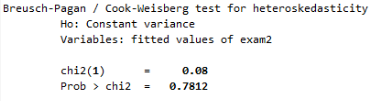
\includegraphics[width=0.3\linewidth]{screenshot006}
%	\caption{Percent deviation from steady state}
%	\label{fig:screenshot006}
%\end{figure}
%
%
























%%%%%%%%%%%%%%%%%%%%%%%%%%%%%%%%%%%%%%%%%%%%%%%%%%%%%%%%%%%%%%%%%%%%%%%%%%%%%%%%%%%%%%%%%%%%%%%%%%%%%%%%%%%%%%%%%%%%%%%%%%%%%%%%%%%%%%%%%%%%

\newpage



%%%%%%% Заключение %%%%%%%




\chapter*{Заключение}
% Добавляем заключение в оглавление
\addcontentsline{toc}{chapter}{Заключение}


%?
%При решении стохастической задачи Рамсея   рабочая сила принимается равной или пропорциональной населению. 
%Но для расширения модели Ramsey-Cass-Koopmans с контролируемым предложением рабочей силы подразумевается  также контролируем рост населения. 
%Очевидно, контроль роста населения - трудная задача, хотя мы знаем  примеры стран с быстрорастущей численностью населения,   проводящих   политику контроля  рождаемости. Этот вопрос остается открытым.

В этом  исследовании  продемонстрированы  важность стохастических свойств экономических переменных  и их применимость к  макроэкономическим  теориям роста.  




В этой работе мы изучили экономический рост при проблеме ограниченности природных ресурсов  в условии  неопределенности.
Используя методы  стохастического анализа мы изучили влияние параметров модели на равновесие для частного случая и сможем сделать это в общем случае с   помощью численных  методов. 



Главным  выводом работы является тот  факт, что добавление неопределенности в модель может привести к  тому, что  при некоторых коэффициентах ресурс будет полностью  исчерпан.    


В итоге мы видим, что раличные  политики могут как положительно повлиять  на запасы ограниченного ресурса, так, наоборот, отрицательно, что приведет к полному исчерпанию ресурса.  
%В качестве подтверждения приведем пример из жизни:   люди  вырубают  деревья, чтобы развивать экономику, что  в то же время приводит к истончению ресурса.  

Выбор оптимальной политики зависит от скорости, с которой экономика  сходится  к устойчивому состоянию, ставки межвременного дисконтирования, вогнутости предпочтений и т.д.  

Реальные данные могут сильно отличаться от предсказаний  математических моделей. В любом случае хорошая модель это не та, которая позволяет   описывает все возможные экономики,  а та,  которая позволяет   воспроизвести некоторый аспект  реальности для оценки эффективности введения какой-либо реальной политики.


Вообще, факторы ограничивающие темпы   роста зависят от   многих  аспектов жизни общества,  включая демографические, экологические, социальные  и политические. Обычно эти процессы исключаются из формального анализа моделей для  значительного их  упрощения, что ограничивает  возможность экономической теории объяснить причину  отклонений  эмпирических данных от гипотетических моделей.  

Это важная область  для экономического анализа, и исследования в ней необходимо продолжить.


 




%%%%%%%%%%% Список литературы	%%%%%%%%%%%


\nocite{*}  %Чтобы в список литературы напечаталичь все источники из bib-файла

% Если нам хочется, чтобы в списке литературы были не полуторные интервалы можно воспользоваться следующим приёмом:
\begingroup
\setstretch{1}
\addcontentsline{toc}{chapter}{Список литературы}
\printbibliography[title = {Список литературы}]
\endgroup



%%%%%%%%%%%%%%%%%%%% Приложения %%%%%%%%%%%%%%%%%%%%

\appendix
\renewcommand{\thechapter}{\Asbuk{chapter}}

%%%%%%%%%% titlesec для приложений
\titleformat{\chapter}
 {\normalfont\bfseries\large}{\chaptertitlename~\thechapter}{0.25em}{\normalfont}


\titlecontents{chapter}
              [0 em] %
              {\normalsize}
              {\makebox[7em][l]{Приложение \thecontentslabel}}
              {Приложение }
              {\titlerule*[10pt]{.}\contentspage}


\chapter{Обзор  теорий экономического роста}




\begin{longtable}
	{   >{\centering\footnotesize}p{6em}
		>{\centering\footnotesize}p{15em}
		>{\centering\footnotesize\arraybackslash}p{15em}
	}
	\caption{Краткий обзор основных моделей  экономического роста}\label{ltab}\\
	
	\hline
	Модель  	  & Ключевые элементы  & Основные результаты \\\hline 
	\endfirsthead
	
	\multicolumn{3}{r}{Продолжение таблицы \ref{ltab}}\\\hline
	Модель  	  & Ключевые элементы  & Результат \\\hline
	\endhead
	
	\multicolumn{3}{r}{Окончание таблицы \ref{ltab}}\\\hline
	Модель  	  & Ключевые элементы  & Результат  \\\hline
	\endlasthead
	
	\multicolumn{3}{c}{\footnotesize Классическая экономическая теория} \\
	
	
	А. Смит (1776) &  Накопление капитала, рост рабочей силы  и разделение труда  & 
	Повышение эффективности использования капитала путем разделения труда и технического прогресса. Продвижение внешней торговли для  расширения рынка и укрепления  источников экономического  роста 
	\\
	
	Т. Мальтус (1798) & Экономический рост при росте населения  &
	Темпы роста падают при увеличении 	населения 	
	\\
	
	Д. Рикардо  (1817) &  Закон уменьшающейся отдачи от факторов  роста  & 	  Причиной  снижения качества ресурсов является закон убывающей отдачи, а не их абсолютная  нехватка \\ 
	
	
	Дж. М. Кейнс (1923)   &   Привлечение инвестиций  & Низкие процентные ставки, государственные инвестиции и перераспределение богатства 
	\\ 
	
	\hline
	\multicolumn{3}{c}{\footnotesize Неоклассические  модели экономического роста} \\
	
	
	Модель Харрода—Домара (1939) &   Рост зависит от количества рабочей силы и капитала,  экзогенно определяется нормой сбережений  &
	Стимулирование роста с помощью  инвестиций путем  увеличения  нормы  сбережения и применения достижений   технологического прогресса 
	\\
	
	Модель Солоу — Суона (1956) & 
	Долгосрочный  рост зависит от накопления капитала,  рабочей силы или населения,  роста  производительности (технологический прогресс).  	& 
	Технологический прогресс нейтрален к эффектам  масштаба. Сдвиги в производственной функции не влияют на предельные нормы   замещения при данных соотношениях капитала к труду.	 \\
	
	Модель Солоу с человеческим капиталом (Mankiw-Romer-Weil, 1992)  & 
	Экономические агенты  одинаково  инвестируют как в человеческий капитал, так и  в физический капитал. 
	Нормы сбережения, темпы роста населения и технического прогресса экзогенно заданы.	 	& 
	Экономика  сходится к устойчивому  состоянию, пока уровни физического и человеческого капитала  на одного работника растут. 
	Человеческий капитал обесценивается так  же, как и физический  с  постоянным темпом $ \delta $.
	\\ 
	
	
	Модель Рамсея-Касса-Купманса (1965) & 
	Сбережения больше не являются экзогенными: оптимальные пути потребления и сбережения определяются из взаимодействия  домохозяйствами и фирм на конкурентных рынках.  &  
	Объяснение основных экономических закономерностей, но не самих причин  роста, поскольку  темпы роста рабочей силы в модели   заданы экзогенно. 
	\\
	
	Модель Брока-Мирмана  (1972)	 & 
	Обобщенная на стохастический случай модель неоклассического роста. Понятие устойчивого состояния в стохастическом смысле определено с помощью  порожденных стохастическим процессом роста функций распределения коэффициентов отношения капитала к труду. 	  &
	Для каждой допустимой политики соответствующая стохастическая система имеет единственное  стационарное состояние, которое является вырожденным распределением в детерминированной теории. Это  распределение  устойчиво в том смысле, что множество возможных состояний системы  сходится к  определенному множеству, аналогу детерминированного стационарного состояния. 
	\\
	
	Теория реального делового цикла (1982)  & 
	Модель  используемая  для количественного анализа  бизнес-циклов. 
	& Технологические шоки  объясняют большую часть динамики  бизнес-циклов. \\
	
	\hline
	\multicolumn{3}{c}{\footnotesize Модели  эндогенного роста} \\
	
	Модель AK (1980) & Двигателем  роста является производственная функция с  постоянной отдачей от   масштаба, причем отсутствует эффект  уменьшающейся отдачи капитала  &   Существует аналог AK модели, AH модель, где вместо физического  капитала фактором роста является человеческий капитал  \\  
	
	
	Модель Узавы — Лукаса (1990) & 
	Двухсекторная модифицированная  модель АК, в которой физический и человеческий капитал производятся двумя  различными технологиями.
	Темп роста человеческого капитала  зависит от распределения  приобретения навыков работниками по времени.
	&
	Установившиеся темпы роста зависят  от темпов роста человеческого капитала, предпочтений и от политики, влияющей на  частные стимулы  для инвестиций в любую форму капитала. 
	\\
	
	
	Модель Ромера  (1990)   & 
	Модифицированная модель AK долгосрочного экономического роста, основывающаяся на результатах  научных исследований,  возрастающей отдаче от факторов производства. 	
	Главные двигатели роста: 	 идеи,  отсутствие соперничества  и несовершенная конкуренция.
	&
	Создание новых знаний одной фирмой оказывает положительный внешний эффект  на производственные возможности других фирм.
	Снижение  отдачи от человеческого и физического капитала не происходит из-за экстерналий, и, следовательно, основная причина  конвергенции исчезает.
	\\
	
	Модель Bewley-Hugget-Aiyagari  (1983) &  
	В модель вводятся неполные  рынки с континуумом  идентичных агентов, строящих  прогнозы на будущее.  Агенты решают проблему оптимального  потребления на бесконечном горизонте. 
	& 
	Доход агентов определяется  состоянием системы, которая  задается   стохастически, а потому  и  доходы агентов описываются   стохастическим  процессом.	 
	\\ 
	
	\hline
	\multicolumn{3}{c}{\footnotesize Модели экономического  развития } \\
	
	Двухсекторная модель Льюиса  (1954)   &  
	Механизм изменения структуры слаборазвитых экономик  от  сельского хозяйства  к более  урбанизированным системам
	&
	Два  типа экономик сосуществуют и являются связанными  друг с другом
	\\
	
	
	Теория стадий экономического роста Ростоу (1959) & 
	Все страны проходят несколько этапов развития в процессе экономического роста
	&
	Модель объясняет эмпирические закономерности,  хотя    и  является достаточно механической, поскольку не понятно,  что является основной причиной роста, поэтому модель скорее полезна для классификации.
	\\
	
	
	Модель Шумпетера (1926)   &
	«Созидательное  разрушение» как  причина  инноваций. 
	Фирма  улучшает качество продукции за счет инноваций в то время, как  конкуренты теряют рыночную силу, 
	поскольку инновации создают  более продуктивный промежуточный товар, из-за которого   ранее доступный товар  становится  устаревшим.		
	&  
	Главным фактором  роста являются   инновации и технический прогресс, а не накопление капитала.   	
	Различие между экономическим ростом и развитием.  
	Развитие происходит не постепенно, а циклично после применения инноваций.  
	\\\hline
\end{longtable}





% \begin{Enumerate}  1. Нумерованный список, содержащий в одном пункте несколько предложений

% \begin{enumerate}  1) Приведем пример нумерованного списка, содержащего в одном пункте одно предложение:

% Двухуровневый нумерованный список:
%	\begin{twoenumerate}
%		\item а) тест списка начинается с маленькой буквы и заканчивается точкой с запятой;
%			\begin{twoenumerate}
%				\item 1) текст списка выравнивается по ширине;
%			\end{twoenumerate}
%		\item последнее предложение оканчивается точкой.
%	\end{twoenumerate}

% \begin{itemize}  - Ненумерованные списки используются для перечислений:


% Ссыыылка  По структуре доклад можно разделить на три части\footnote{Аристер Н.И.}. 

%Таблица
%
%\begin{table}[H]
%\caption{Матрица $X$ исходных данных для решения задачи выбора вариантов данных}\label{tab:02:01}
%  \centering
%\begin{tabular}%{\linewidth}
%{|c|c|c|c|c|c|c|c|}\hline
%1	& $x_{11}$ & $x_{12}$ & ... & $x_{1j}$ & ... & $x_{1,m-1} $ & $x_{1,m}$\\\hline
%2	& $x_{21}$ & $x_{22}$ & ... & $x_{2j}$ & ... & $x_{2,m-1} $ & $x_{2,m}$\\\hline
%\end{tabular}
%\end{table}


\end{document}
